\section{Conservation Tracking}

\begin{frame}{Conservation Tracking - Graphical Model}
    \begin{figure}
        \centering
        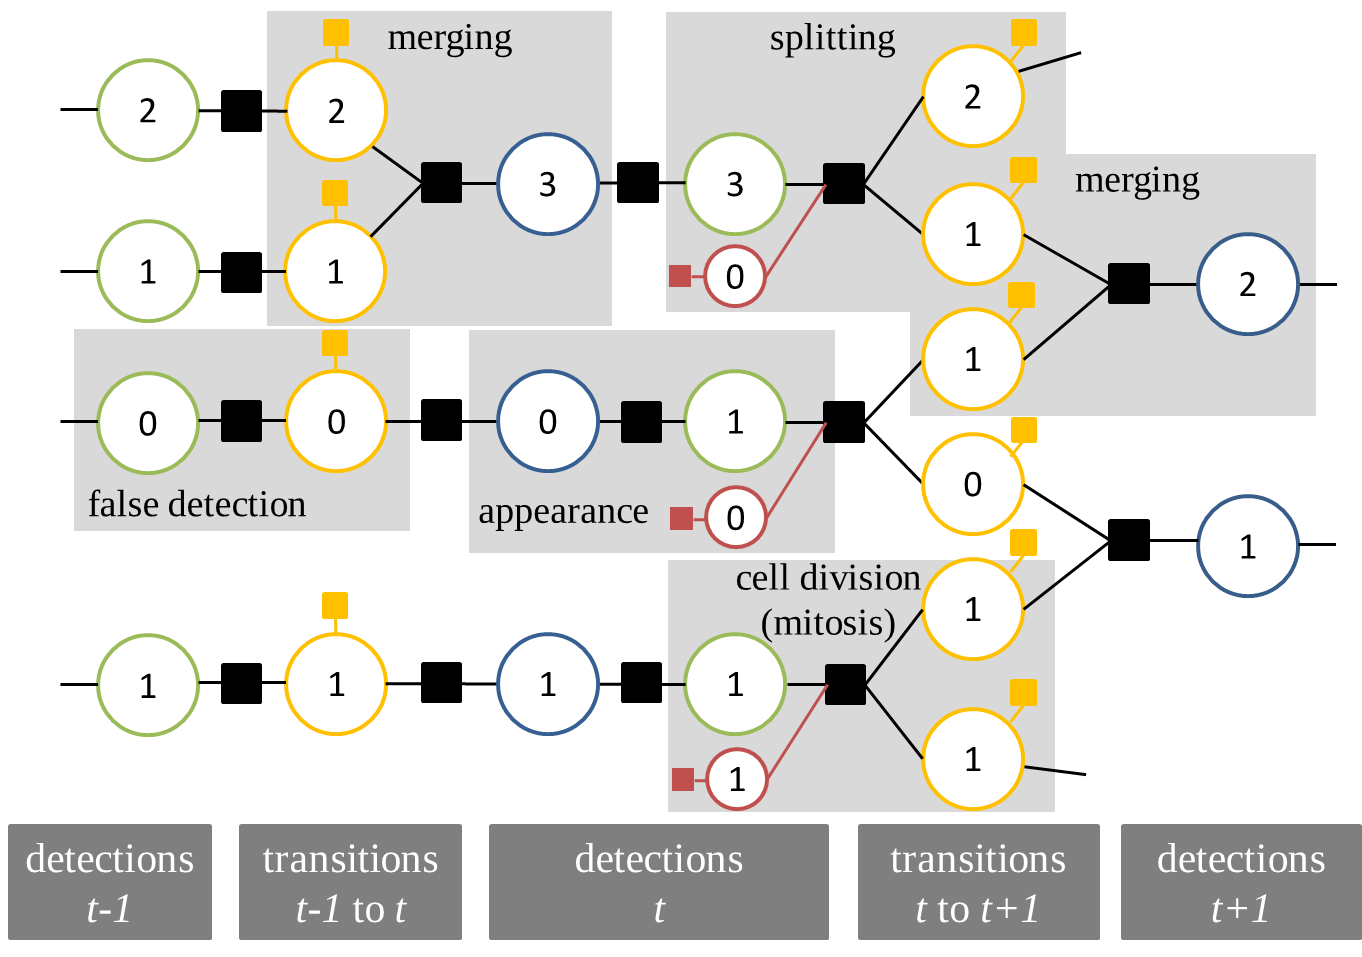
\includegraphics[width=0.8\textwidth]{images/conservation/factor_graph_big3.png}
        \caption{[Schiegg \etal (2013): Conservation Tracking]}
    \end{figure}
\end{frame}

\begin{frame}{Merger Detection and Resolution - Basic Idea}
    \begin{tikzpicture}
        \node[label=left:$t\phantom{+1}$] (s1)
        {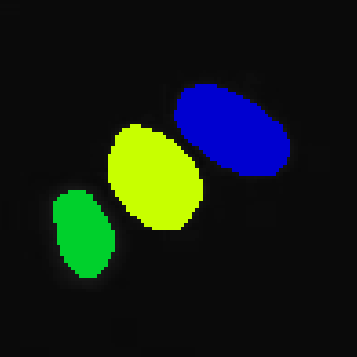
\includegraphics[width=0.17\textwidth]{images/conservation/concept/chaingraph-01.png}};
        \node[label=left:$t+1$, below=of s1.center] (s2)
        {
\includegraphics[width=0.17\textwidth]{images/conservation/concept/chaingraph-02.png}};
        \node[label=left:$t+2$, below=of s2.center] (s3)
        {
\includegraphics[width=0.17\textwidth]{images/conservation/concept/chaingraph-03.png}};
        \node[above=of s1.center] {Segmentation};
        \uncover<2->{
            \node[right=of s1.center, xshift=12pt] (t1)
            {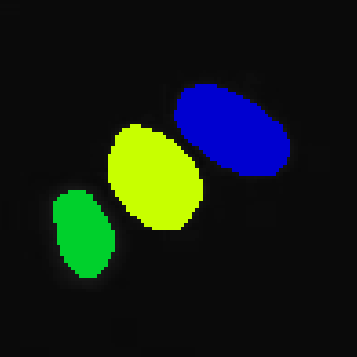
\includegraphics[width=0.17\textwidth]{images/conservation/concept/constracking-01.png}};
            \node[ below=of t1.center] (t2)
            {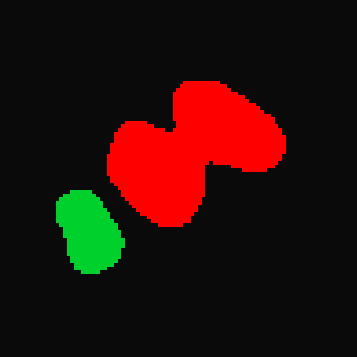
\includegraphics[width=0.17\textwidth]{images/conservation/concept/constracking-02.png}};
            \node[below=of t2.center] (t3)
            {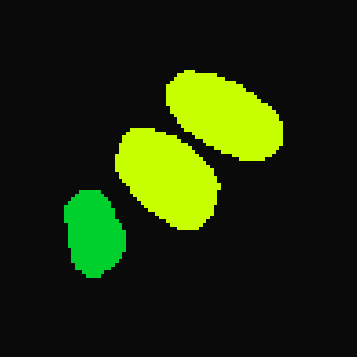
\includegraphics[width=0.17\textwidth]{images/conservation/concept/constracking-03.png}};
            \node[above=of t1.center] {Tracking};
            \node[font=\boldmath, yshift=2pt] at (t2.center) {$2$};
            \begin{scope}[overlay]%
                \uncover<3->{
                    \node[circle, draw=red!90, ultra thick, xshift=4, yshift=4,
                    label={[xshift=-3,color=red!90]right:{\Huge{\xmark}}}]
                    at (t3.center) {\phantom{$BLA$}};
                }
            \end{scope}
        }
        \uncover<4->{
            \node[right=of t1.center, xshift=12pt] (m1)
            {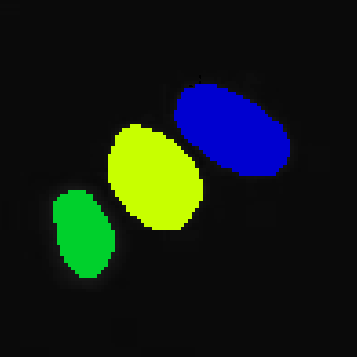
\includegraphics[width=0.17\textwidth]{images/conservation/concept/resolution-01.png}};
            \node[ below=of m1.center] (m2)
            {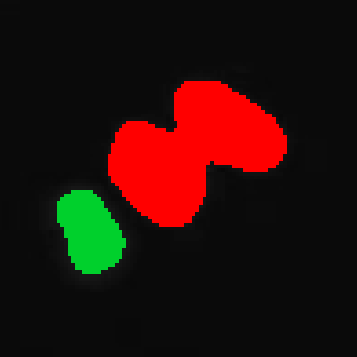
\includegraphics[width=0.17\textwidth]{images/conservation/concept/resolution-02.png}};
            \node[below=of m2.center] (m3)
            {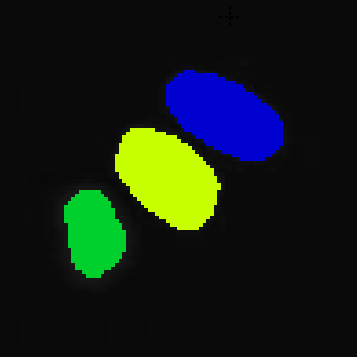
\includegraphics[width=0.17\textwidth]{images/conservation/concept/resolution-03.png}};
            \node[above=of m1.center, align=center] (rm) {Resolved\\Mergers};
            \visible<4>{
                \node[font=\boldmath, yshift=2pt] at (m2.center) {$2$};
            }
            \begin{scope}[overlay]%
                \uncover<5->{
                    \node[ellipse, draw=blue, ultra thick, rotate=-30,
                    xshift=3.2,yshift=11.2,scale=0.55] at (m2.center)
                    {\phantom{$BLA$}};
                    \node[ellipse, draw=yellow, ultra thick, rotate=-45,
                    xshift=-3.2,yshift=-1.2,scale=0.65] at (m2.center)
                    {\phantom{$BL$}};
                }
                \uncover<6->{
                    \node[circle, draw=green!90, ultra thick, xshift=4, yshift=4,
                    label={[xshift=-3,color=green!90]right:{\Huge{\cmark}}}]
                    at (m3.center) {\phantom{$BLA$}};
                }
                
                \begin{scope}[on background layer]
                    \uncover<7->{
                        \node[rectangle, draw=OrangeRed!95, ultra thick, fit=(rm) (m3)] (rect) {};
                        \node[arrowstyle=2,rotate=180,xshift=-45,scale=0.8] at (rect.east) {\rotatebox{180}{My
                                Contribution}};
                    }
                \end{scope}
            \end{scope}
        }
    \end{tikzpicture}
\end{frame}

\begin{frame}{Conservation Tracking - Workflow with Merger Resolution}
    \begin{figure}
        \centering
        \begin{tikzpicture}
            \node[anchor=south west, inner sep=0] (image) at (0,0)
            {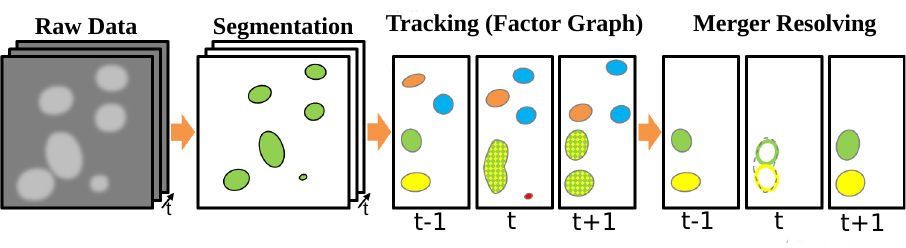
\includegraphics[width=\textwidth]{images/conservation/pipeline_no_preprocessing.png}};
            \begin{scope}[x={(image.south east)},y={(image.north west)}]
                \draw[red,line width=2pt,rounded corners, fill=red!20, fill opacity=0.3]
                (0.728,0.04) rectangle (1.003,0.97);
            \end{scope}
        \end{tikzpicture}

        \label{fig:conservation-pipeline}
    \end{figure}
\end{frame}



\begin{frame}{Merger Resolution - Gaussian Mixture Model}
    \begin{figure}
        \centering
        \begin{subfigure}[b]{0.44\textwidth}
            \centering
            \scalebox{0.74}{
                % \begin{tikzpicture}
% \tikzstyle{main}=[circle, minimum size = 10mm, thick, draw =black!80, node distance = 16mm]
% \tikzstyle{hyparam}=[rectangle, minimum size = 5mm, thick, draw =black!80, fill = black!10, node distance = 16mm]
% \tikzstyle{param}=[rectangle, minimum size = 5mm, thick, draw =black!80, node distance = 16mm]
% \tikzstyle{connect}=[-latex, thick]
% \tikzstyle{selector}=[-latex, -|, snake=snake,segment amplitude=.4mm,segment length=2mm,line after snake=1mm, thick]
% \tikzstyle{shortconnect}=[-latex, thin]
% \tikzstyle{box}=[rectangle, draw=black!100]
% \tikzstyle{switch}=[circle, minimum size = 1mm, fill = black!100, draw=black!100]
%   \node[param] (phi) [label=below:$p(h)$] {$[H]$};
%   \node[main] (z) [right of=phi,label=below:$h^n$] {K};
%   \node[param] (mu) [above of=phi,yshift=10mm, label=below:$\MUH$] { };
%   \node[main, fill = black!10] (x) [right of= z,label=below:$v^n$] { };
%   \node[param] (sigma) [above of=z,yshift=10mm, label=right:$\SIGMAH$] { };
%   \path (phi) edge [connect] (z)
%         (z) edge [selector] (x)
%         (mu) edge [connect] (x)
%         (sigma) edge [connect] (x);
%   \node[rectangle, inner sep=0mm, fit= (z) (x),label=below right:$N$, xshift=9mm] {};
%   \node[rectangle, inner sep=4.4mm,draw=black!100, fit= (z) (x), xshift=1mm] {};
%   \node[rectangle, inner sep=2mm, fit= (mu) (sigma),label=below right:$H$, yshift=-2mm, xshift=11mm] {};
%   \node[rectangle, inner sep=6.4mm,draw=black!100, fit= (mu) (sigma), yshift=-2mm, xshift=3mm] {};
% \end{tikzpicture}

\begin{tikzpicture}
  \node[param] (pi) [] {$\Pi$};
  \node[main] (z) [right of=pi,label=below:$h^n$] { };
  \node[param] (mu) [above of=pi,yshift=10mm, label=below:$\MUH$] { };
  \node[main, fill = black!30] (x) [right of= z,label=below:$v^n$] { };
  \node[param] (sigma) [above of=z,yshift=10mm, label=right:$\SIGMAH$] { };
  \path (pi) edge [connect] (z)
        (z) edge [connect] (x)
        (mu) edge [connect] (x)
        (sigma) edge [connect] (x);
  \node[rectangle, inner sep=0mm, fit= (z) (x),label=below right:N, xshift=9mm] {};
  \node[rectangle, inner sep=4.4mm,draw=black!100, fit= (z) (x), xshift=1mm] {};
  \node[rectangle, inner sep=2mm, fit= (mu) (sigma),label=below right:H, yshift=-2mm, xshift=11mm] {};
  \node[rectangle, inner sep=6.4mm,draw=black!100, fit= (mu) (sigma), yshift=-2mm, xshift=3mm] {};
\end{tikzpicture}



%%% Local Variables: 
%%% mode: latex
%%% TeX-master: "../../main"
%%% End: 

            }
            \caption{GMM - plate notation.}
        \end{subfigure}
        \hfill
        \begin{subfigure}[b]{0.44\textwidth}
            \centering
            \scalebox{0.65}{
                \tdplotsetmaincoords{60}{110}

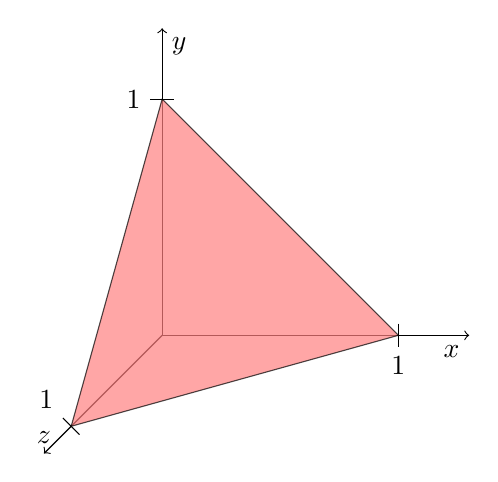
\begin{tikzpicture}[scale=3]
    \begin{scope}
        \draw[->] (0,0,0) -- (1.3,0,0) node[anchor=north east]{$x$};
        \draw[->] (0,0,0) -- (0,1.3,0) node[anchor=north west]{$y$};
        \draw[->] (0,0,0) -- (0,0,1.3) node[anchor=south]{$z$};
        \draw [fill=red!50, opacity=0.7] (0,0,1)--(1,0,0)--(0,1,0)--cycle;
        \draw (1,0.05,0) -- (1,-0.05,0) node[anchor=north]{$1$};
        \draw (0.05,1,0) -- (-0.05,1,0) node[anchor=east] {$1$};
        \draw (0.035,-0.035,1) -- (-0.035,0.035,1) node[anchor=south east]{$1$};
        
    \end{scope}
\end{tikzpicture}

%%% Local Variables: 
%%% mode: latex
%%% TeX-master: "../../main"
%%% End: 

            }
            \caption{Convex Combination.}
        \end{subfigure}
        \label{fig:conservation-gmm}
    \end{figure}
    \begin{align*}
        p(v) = \sum_{h=1}^H\pi_h\cdot\mathcal{N}({v}|\MUH , \SIGMAH )
        % \mathsmaller{p(v)} &= \mathsmaller{\mathcal{N}({v}|\MUH , \SIGMAH )} \\ 
        % &\mathsmaller{= \frac{1}{\sqrt{\det(2\pi\SIGMAH )} }\exp\left(-\frac{1}{2}({v}-\MUH )^\intercal
        %     \left(\SIGMAH\right) ^{-1} ({v}-\MUH )\right)}
    \end{align*}
\end{frame}



\begin{frame}{Merger Resolution - Experimental Results}
    \begin{table}
        \centering
        \def\arraystretch{0.5}
\newlength\tablemathtext
\settototalheight\tablemathtext{\parbox{\linewidth}{$t=75$, $\id=446$}}
% \setlength{\tabcolsep}{1pt}
\scalebox{0.95}{
    \begin{tabular}{lccc}
        \toprule
        Time Step \& Id  & Raw Data & Segmentation & GMM fit \\ \midrule
        $t=75$, $\id=446$&
        \raisebox{\tablemathtext-\height}{
            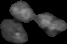
\includegraphics[width=0.18\textwidth]{images/conservation/t=75,id=446,k=3_raw.png}} &
        \raisebox{\tablemathtext-\height}{
            
\includegraphics[width=0.18\textwidth]{images/conservation/t=75,id=446,k=3_label.png}} &
        \raisebox{\tablemathtext-\height}{
            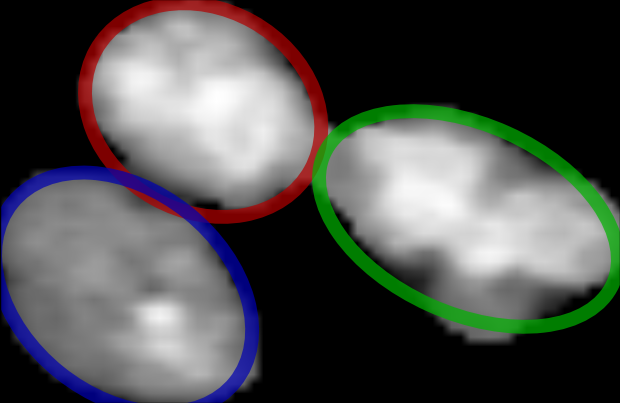
\includegraphics[width=0.18\textwidth]{images/conservation/t=75,id=446,k=3_fit.png}} \\
        &&& \\
        $t=75$, $\id=206$&
        \raisebox{\tablemathtext-\height}{
            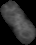
\includegraphics[width=0.18\textwidth]{images/conservation/t=75,id=206,k=2_raw.png}} &
        \raisebox{\tablemathtext-\height}{
            
\includegraphics[width=0.18\textwidth]{images/conservation/t=75,id=206,k=2_label.png}} &
        \raisebox{\tablemathtext-\height}{
            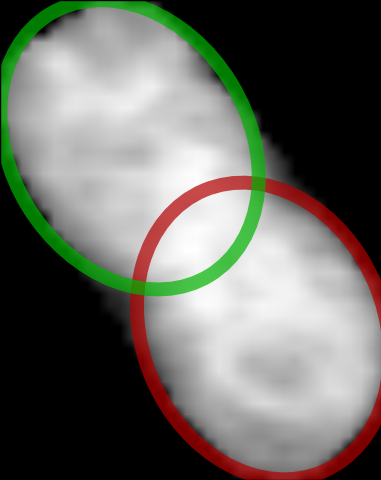
\includegraphics[width=0.18\textwidth]{images/conservation/t=75,id=206,k=2_fit.png}} \\
        &&& \\
        $t=85$, $\id=334$&
        \raisebox{\tablemathtext-\height}{
            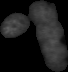
\includegraphics[width=0.18\textwidth]{images/conservation/t=85,id=334,k=4_raw.png}} &
        \raisebox{\tablemathtext-\height}{
            \hspace{-3pt}
\includegraphics[width=0.18\textwidth]{images/conservation/t=85,id=334,k=4_label.png}} &
        \raisebox{\tablemathtext-\height}{
            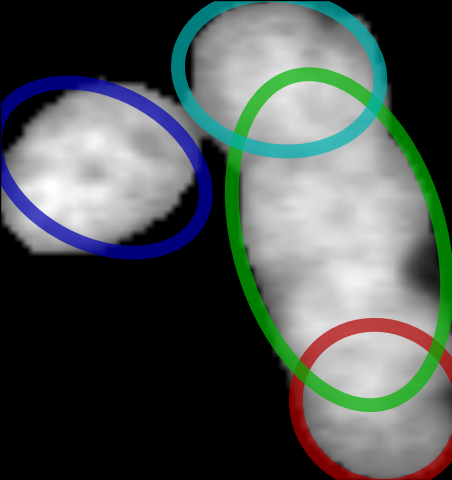
\includegraphics[width=0.18\textwidth]{images/conservation/t=85,id=334,k=4_fit.png}} \\
        \bottomrule
    \end{tabular}
}
\def\arraystretch{1.0}

% WHY THE FUCK THE NEED FOR NEGATIVE HSPACE IN LAST ROW?



%%% Local Variables: 
%%% mode: latex
%%% TeX-master: "../../main"
%%% End: 

        \caption{GMM fits to merged objects.}
        \label{tab:conservation-gmm-fits}
    \end{table}
\end{frame}


\begin{frame}{Conservation Tracking with Merger Resolution - Experimental Results}
    \begin{table} % \small % \hfill{} \centering
        \scalebox{0.8}{
            \begin{tabular}{l||ccc|ccc}
                \toprule
                & \multicolumn{3}{c|}{\textbf{Moves}} & \multicolumn{3}{c}{\textbf{Divisions}} \\
                & Precision& Recall& $\fmeasure$ & Precision& Recall& $\fmeasure$ \\ \hline
                Kausler \etal & 0.99 & 0.97 & 0.98 & 0.65 & 0.68 & 0.66 \\
                Classifiers only & \textit{N/A} & \textit{N/A} & \textit{N/A} & 0.92 & 0.56 & 0.70 \\
                Ours ($m=1$)\footnote{\color{red}m: the maximum number of merged objects per connected component} & 0.99 & 0.97 & 0.98 & 0.68 & 0.71 & 0.70 \\
                Ours ($m=2$) & 1.00 & 0.99 & 0.99 & 0.85 & 0.76 & 0.80 \\
                Ours ($m=3$) & 1.00 & 0.99 & 0.99 & 0.85 & 0.77 & 0.80 \\
                Ours ($m=4$) & 1.00 & 0.99 & 0.99 & 0.85 & 0.76 & 0.80 \\
                \midrule & \multicolumn{3}{c|}{\textbf{Mergers} } & \multicolumn{3}{c}{\textbf{Resolved Mergers}} \\ 
                & Precision& Recall& $F_{1}$ & Precision& Recall& $F_{1}$ \\ \hline
                Kausler \etal & \textit{N/A}& \textit{N/A} & \textit{N/A} & \textit{N/A}&
                \textit{N/A} & \textit{N/A} \\
                Classifiers only & 0.41 & 0.62 & 0.49 & \textit{N/A}& \textit{N/A} & \textit{N/A} \\
                Ours ($m=1$) & \textit{N/A}& \textit{N/A} & \textit{N/A} & \textit{N/A}& \textit{N/A} & \textit{N/A}\\ 
                Ours ($m=2$) & 0.73 & 0.60 & 0.66 & 0.79 & 0.70 & 0.74\\
                Ours ($m=3$) & 0.84 & 0.69 & 0.76 & 0.85 & 0.75 & 0.79\\
                Ours ($m=4$) & 0.84 & 0.69 & 0.76 & 0.85 & 0.75 & 0.80\\
                \bottomrule
            \end{tabular}
        }
        % \caption{Results for Mitocheck data set.}
        \label{tab:gmm-result-c}
    \end{table}
\end{frame}



%%% Local Variables: 
%%% mode: latex
%%% TeX-master: "../main"
%%% End: 
